\documentclass{beamer}

\mode<presentation> {

% The Beamer class comes with a number of default slide themes
% which change the colors and layouts of slides. Below this is a list
% of all the themes, uncomment each in turn to see what they look like.

%\usetheme{default}
%\usetheme{AnnArbor}
%\usetheme{Antibes}
%\usetheme{Bergen}
%\usetheme{Berkeley}
%\usetheme{Berlin}
%\usetheme{Boadilla}
%\usetheme{CambridgeUS}
%\usetheme{Copenhagen}
%\usetheme{Darmstadt}
%\usetheme{Dresden}
\usetheme{Frankfurt}
%\usetheme{Goettingen}
%\usetheme{Hannover}
%\usetheme{Ilmenau}
%\usetheme{JuanLesPins}
%\usetheme{Luebeck}
%\usetheme{Madrid}
%\usetheme{Malmoe}
%\usetheme{Marburg}
%\usetheme{Montpellier}
%\usetheme{PaloAlto}
%\usetheme{Pittsburgh}
%\usetheme{Rochester}
%\usetheme{Singapore}
%\usetheme{Szeged}
%\usetheme{Warsaw}

% As well as themes, the Beamer class has a number of color themes
% for any slide theme. Uncomment each of these in turn to see how it
% changes the colors of your current slide theme.

%\usecolortheme{albatross}
%\usecolortheme{beaver}
%\usecolortheme{beetle}
\usecolortheme{crane}
%\usecolortheme{dolphin}
%\usecolortheme{dove}
%\usecolortheme{fly}
%\usecolortheme{lily}
%\usecolortheme{orchid}
%\usecolortheme{rose}
%\usecolortheme{seagull}
%\usecolortheme{seahorse}
%\usecolortheme{whale}
%\usecolortheme{wolverine}

%\setbeamertemplate{footline} % To remove the footer line in all slides uncomment this line
%\setbeamertemplate{footline}[page number] % To replace the footer line in all slides with a simple slide count uncomment this line

%\setbeamertemplate{navigation symbols}{} % To remove the navigation symbols from the bottom of all slides uncomment this line
}

\usepackage{units}
\usepackage{extpfeil}
\usepackage{extarrows} %Allows long equation signs
\usepackage{graphicx} % Allows including images
\usepackage{booktabs} % Allows the use of \toprule, \midrule and \bottomrule in tables
\usepackage{physics}
\usepackage{tikz}
\usepackage{cite}
%花体字母
\usepackage{amsthm,amsmath,amssymb}
\usepackage{mathrsfs}
\usepackage{dutchcal}
\usepackage{circuitikz}
\usepackage{eqnarray}

%----------------------------------------------------------------------------------------
%	TITLE PAGE
%----------------------------------------------------------------------------------------

\title[VP260 RC]{VP260 Recitation Class 6} % The short title appears at the bottom of every slide, the full title is only on the title page

\author{Yanjun Chen} % Your name
\institute[UM-SJTU JI] % Your institution as it will appear on the bottom of every slide, may be shorthand to save space
{
    University of Michigan - Shanghai Jiao Tong University Joint Institute\\% Your institution for the title page
\medskip
}
\date{\today} % Date, can be changed to a custom date

\begin{document}

\begin{frame}
    \titlepage % Print the title page as the first slide
\end{frame}


%----------------------------------------------------------------------------------------
%	 SECTION 1
%----------------------------------------------------------------------------------------

\section{Fundamental Concepts} % Section title slide, unnumbered

\begin{frame}{Motional emf}
    \begin{columns}
        \begin{column}{0.5\textwidth}
            \begin{figure}[htbp]
                \centering
                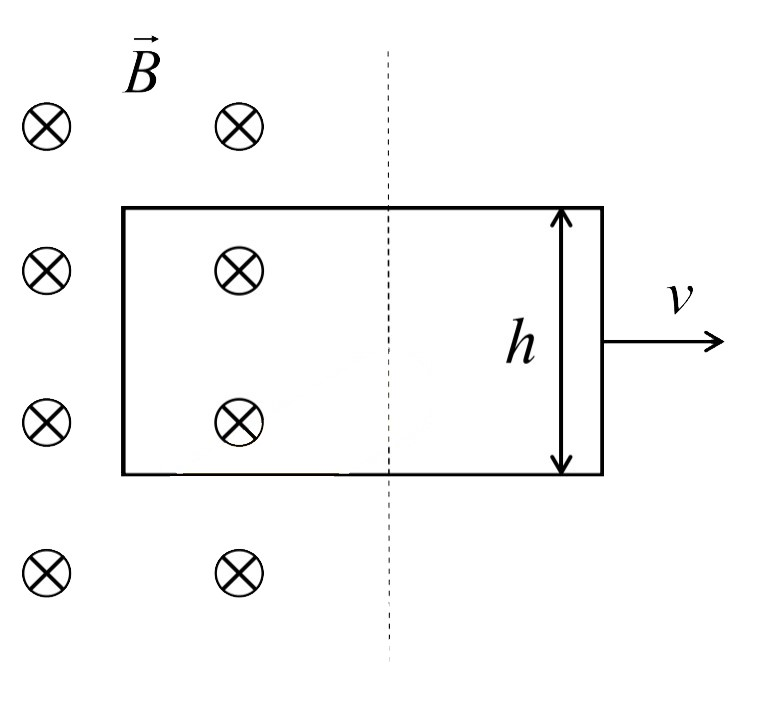
\includegraphics[width=0.7\textwidth]{Images/motional.jpg}
            \end{figure}

            \begin{block}{Motional emf}
                \begin{equation}
                    \varepsilon = \oint \va{F}_{\text{mag}} \vdot \dd{\va{l}} =  v B h
                \end{equation}
            \end{block}
        \end{column}
        \begin{column}{0.5\textwidth}
            We know that,
            \begin{equation}
                \Phi_B = \oint \va{B} \vdot \dd{\va{l}} = Bxh
            \end{equation}
            and,
            \begin{equation}
                \dv{\Phi_B}{t} = Bh\dv{x}{t} = -Bhv = -\varepsilon
            \end{equation}

            \begin{block}{Flux rule for motional emf}
                \begin{equation}
                    \dv{\Phi_B}{t} = -\varepsilon
                \end{equation}
            \end{block}
        \end{column}
    \end{columns}
\end{frame}


\begin{frame}{Faraday’s Law and Lenz' Law}
    A changing magnetic field induces an electric field.
    \begin{equation}
        \varepsilon = \oint \va{E} \vdot \dd{\va{l}} = -\dv{\Phi_B}{t} = -\oint\pdv{\va{B}}{t} \vdot \dd{\va{a}}
    \end{equation}

    \begin{block}{Faraday's law}
        \begin{equation}
            \oint \va{E} \vdot \dd{\va{l}} = -\oint \pdv{\va{B}}{t} \dd{\va{a}}
        \end{equation}

        \begin{equation}
            \curl{\va{E}} = -\pdv{\va{B}}{t}
        \end{equation}
    \end{block}

    \begin{itemize}
        \item The negative sign means that nature abhors a change in flux (Lenz' law).
    \end{itemize}
\end{frame}


\begin{frame}{Induced Electric Field}
    If the charge density is zero and the electric field is induced by changing magnetic field, then
    \begin{align}
        \div{\va{E}} = 0, \qquad & \curl{\va{E}} = -\pdv{\va{B}}{t} \\
        \div{\va{B}} = 0, \qquad & \curl{\va{B}} = \mu_0 \va{J}
    \end{align}

    The electric field is not a conservative field now. So, electric potential is not valid in this field.
\end{frame}


\begin{frame}{Electrodynamics}
    The Ampere's law is,
    \begin{equation}
        \curl{\va{B}} = \mu_0 \va{J}
    \end{equation}
    Take divergence,
    \begin{equation}
        \div{\left( \curl{\va{B}} \right)} = \mu_0\div{\va{J}}
    \end{equation}

    It is not always true that $\div{\va{J}} = 0$.

    \begin{figure}[htbp]
        \centering
        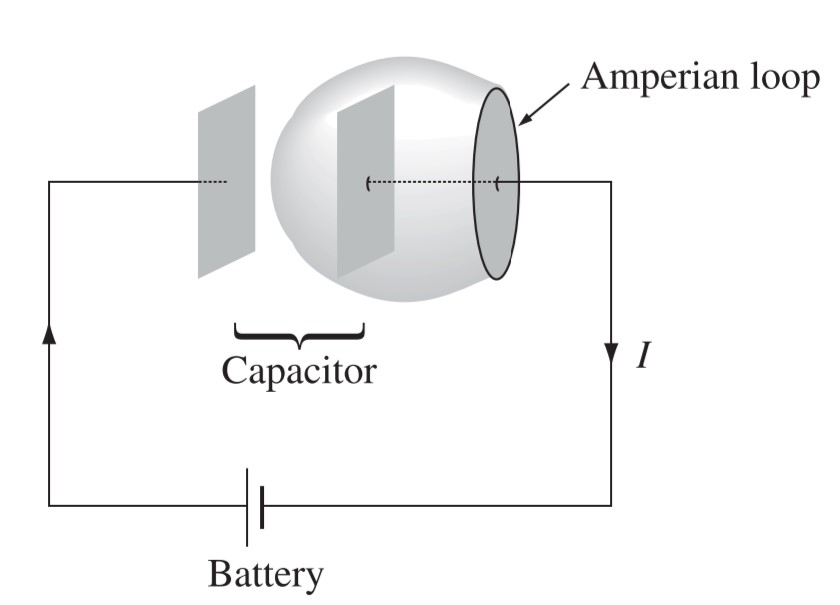
\includegraphics[width=0.6\textwidth]{Images/amp.jpg}
    \end{figure}
\end{frame}

\begin{frame}{Displacement Current}
    We need fix the Ampere's law.

    Consider the continuity equation,
    \begin{equation}
        \div{\va{J}} = -\pdv{\rho}{t}
    \end{equation}

    When the current is not steady ($\div{\va{J}} = 0$),
    \begin{equation}
        \div{\va{J}} = -\pdv{\epsilon_0 \div{\va{E}}}{t}
    \end{equation}

    We put the equation into the Ampere's law, and we get,
    \begin{equation}
        \curl{\va{B}} = \mu_0 \va{J} + \mu_0 \epsilon_0\pdv{\va{E}}{t}
    \end{equation}

    A changing electric field induces a magnetic field.
\end{frame}

\begin{frame}{Displacement Current}
    \begin{block}{Displacement current}
        \begin{equation}
            \va{J}_d = \epsilon_0 \pdv{\va{E}}{t}
        \end{equation}
    \end{block}

    \begin{columns}
        \begin{column}{0.5\textwidth}
            \begin{figure}[htbp]
                \centering
                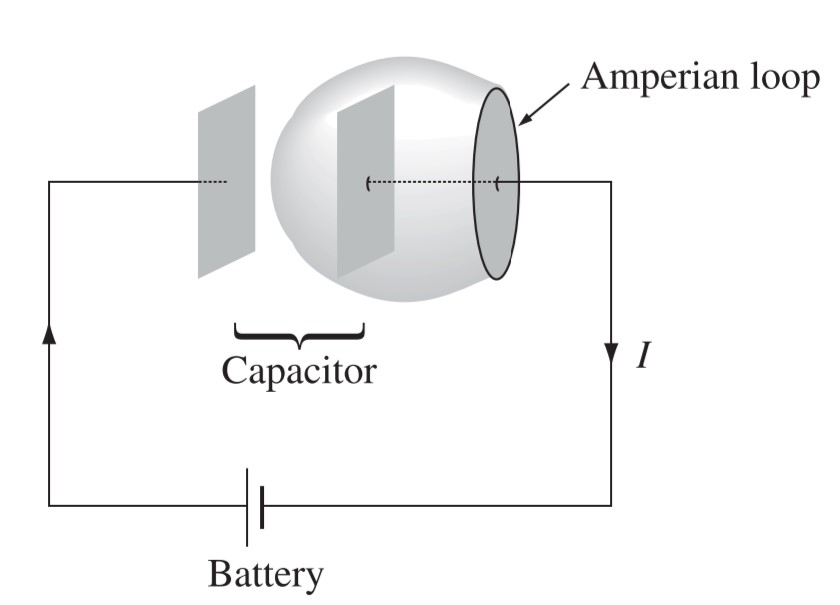
\includegraphics[width=\textwidth]{Images/amp.jpg}
            \end{figure}
        \end{column}
        \begin{column}{0.5\textwidth}
            \begin{equation}
                E = \frac{Q}{\epsilon_0 A}
            \end{equation}

            \begin{equation}
                \epsilon_0 \mu_0 \int \pdv{\va{E}}{t} \vdot \dd{\va{a}} = \mu_0 I
            \end{equation}
        \end{column}
    \end{columns}
\end{frame}

\begin{frame}{Maxwell's Equation}
    \begin{table}[htbp]
        \centering
        \begin{tabular}{ll}
            \toprule
             Integral Form & Differential Form \\
            \midrule
            $\oint \va{E}\vdot\dd{\va{a}}=\frac{Q_{\text{enc}}}{\epsilon_0}$ & $\div{\va{E}} = \frac{\rho}{\epsilon_0}$ \\ \addlinespace
            $\oint \va{E}\vdot\dd{\va{l}}= -\dv{\Phi_B}{t}$ & $\curl{\va{E}}=-\pdv{\va{B}}{t}$ \\ \addlinespace
            $\oint \va{B}\vdot\dd{\va{a}}=0$ & $\div{\va{B}} = 0$ \\ \addlinespace
            $\oint \va{B}\vdot\dd{\va{l}}=\mu_0 I_{\text{enc}} + \mu_0 \epsilon_0 \dv{\Phi_E}{t}$ & $\curl{\va{B}}=\mu_0 \va{J}+ \mu_0 \epsilon_0 \pdv{\va{E}}{t}$             \\
            \bottomrule
        \end{tabular}
    \end{table}
\end{frame}

%----------------------------------------------------------------------------------------
%	 Section 2
%----------------------------------------------------------------------------------------

\section{Exercise}

\begin{frame}{Exercise 1}
  
\end{frame}

\begin{frame}{Exercise 2}
    
\end{frame}

\begin{frame}{Exercise 3}
    
\end{frame}

%----------------------------------------------------------------------------------------
%	 CLOSING/SUPPLEMENTARY SLIDES
%----------------------------------------------------------------------------------------
\section{Appendix}


\begin{frame}
    \begin{center}
        \LARGE\bf Thanks for listening!
    \end{center}
\end{frame}


%----------------------------------------------------------------------------------------

\begin{frame}{\bf References}
    \nocite{*} % Display all references regardless of if they were cited
    \bibliography{example.bib}
    \bibliographystyle{plain}
\end{frame}

\end{document}

